% Table 1 and the CONSORT diagram.
% Copy the disclosure-reviewed table1_current_review.tex into paper/tables/
% (bring it to the current labels with: python -m opera.run.relabel_table1
% paper/tables/table1_current_review.tex), then build with: pdflatex table1_review (x2)
\documentclass[11pt]{article}
\usepackage[a4paper,margin=1.6cm,top=1.4cm,bottom=1.4cm]{geometry}
\usepackage[T1]{fontenc}
\usepackage[utf8]{inputenc}
\usepackage{tgpagella,mathpazo}
\usepackage[scaled=0.95]{helvet}
\usepackage{microtype}
\usepackage{amsmath}
\usepackage{booktabs,tabularx,multirow}
\usepackage{graphicx}
\usepackage[dvipsnames]{xcolor}
\usepackage{caption}
\usepackage{tikz}
\usetikzlibrary{arrows.meta,backgrounds,calc,decorations.pathreplacing,fit,matrix,positioning,shapes.geometric}
\usepackage[hidelinks]{hyperref}
\usepackage[nameinlink,capitalise]{cleveref}
% Shared manuscript and TikZ visual language for the OPERA paper.
% Keep colours and Helvetica-like figure typography synchronized with
% opera/visualization/style.py (Arial/Liberation Sans on render hosts).

\definecolor{OperaIndigo}{HTML}{2D3A8C}
\definecolor{OperaNavy}{HTML}{1A237E}
\definecolor{OperaPeriwinkle}{HTML}{5C7AEA}
\definecolor{OperaSlate}{HTML}{737D8C}
\definecolor{OperaTeal}{HTML}{408579}
\definecolor{OperaGreen}{HTML}{1B7A4A}
\definecolor{OperaSienna}{HTML}{B5451B}
\definecolor{OperaTerracotta}{HTML}{C16A58}
\definecolor{OperaOchre}{HTML}{B18B4D}
\definecolor{OperaLavender}{HTML}{8974AC}
\definecolor{OperaInk}{HTML}{17212B}
\definecolor{OperaInkSecondary}{HTML}{485463}
\definecolor{OperaInkMuted}{HTML}{657180}
\definecolor{OperaBorder}{HTML}{CBD2DA}
\definecolor{OperaGrid}{HTML}{E8ECF1}
\definecolor{OperaPaper}{HTML}{F7F8FA}

\tikzset{
  opera/.style={font=\sffamily\small, text=OperaInk},
  panel/.style={draw=none, fill=white, inner sep=0pt},
  softpanel/.style={
    rounded corners=0.8mm,
    draw=OperaGrid,
    line width=0.45pt,
    fill=OperaPaper,
    inner sep=2.4mm,
  },
  stage/.style={
    rounded corners=0.7mm,
    draw=OperaBorder,
    line width=0.6pt,
    fill=white,
    align=center,
    minimum height=8mm,
    inner xsep=3mm,
    inner ysep=1.8mm,
  },
  stageblue/.style={stage, draw=OperaIndigo!55, fill=OperaIndigo!7},
  stageteal/.style={stage, draw=OperaTeal!65, fill=OperaTeal!8},
  stagewarm/.style={stage, draw=OperaSienna!60, fill=OperaSienna!7},
  latent/.style={
    circle,
    draw=OperaIndigo!65,
    fill=OperaIndigo!9,
    line width=0.6pt,
    minimum size=6mm,
    inner sep=0pt,
    font=\sffamily\scriptsize\bfseries,
  },
  token/.style={
    rounded corners=0.7mm,
    draw=OperaBorder,
    fill=white,
    minimum width=6.2mm,
    minimum height=4.8mm,
    inner sep=0.5mm,
    font=\sffamily\tiny,
    align=center,
  },
  outcome/.style={
    rounded corners=1mm,
    draw=OperaTerracotta!70,
    fill=OperaTerracotta!9,
    minimum height=5.8mm,
    inner xsep=1.8mm,
    font=\sffamily\scriptsize,
    align=center,
  },
  flow/.style={
    -{Latex[length=2mm,width=1.2mm]},
    line width=0.75pt,
    draw=OperaInkSecondary,
  },
  flowblue/.style={flow, draw=OperaIndigo},
  flowteal/.style={flow, draw=OperaTeal},
  flowwarm/.style={flow, draw=OperaSienna},
  relation/.style={
    -{Latex[length=1.8mm,width=1.1mm]},
    line width=0.65pt,
    draw=OperaLavender,
    densely dashed,
  },
  captionnote/.style={
    font=\sffamily\fontsize{6.6}{7.5}\selectfont,
    text=OperaInkMuted,
    align=center,
  },
  labelsmall/.style={
    font=\sffamily\fontsize{7}{8}\selectfont,
    text=OperaInkSecondary,
    align=center,
  },
  heading/.style={
    font=\sffamily\fontsize{9}{10}\selectfont\bfseries,
    text=OperaInk,
    align=left,
  },
  panelletter/.style={font=\sffamily\bfseries\normalsize, text=OperaInk},
  divider/.style={draw=OperaBorder, line width=0.45pt},
  eyebrow/.style={font=\sffamily\fontsize{6.5}{7.5}\selectfont\bfseries,
    text=OperaIndigo, align=left},
}

\newcommand{\placeholder}[1]{\textcolor{OperaSienna}{\textbf{[#1]}}}
\pagestyle{empty}
% The footnote points to the paper's supplementary index table, not part of this sheet.
\newcommand{\indextableref}{table of prognostic indices}

\begin{document}
\renewcommand{\cref}[1]{\indextableref}
\IfFileExists{tables/table1_current_review.tex}
  {% Generated by opera.run.format_table1_release from export sha256 b19cf510d55a662b8e42fbfe9f4a494712762273b4e8ace6e5c97c5d2038bab6 (disclosure policy: primary-only).
% Do not edit values by hand; regenerate from the reviewed export.
\begin{table*}[p]
\centering
\caption{\textbf{Baseline characteristics at first-line treatment.} One record per patient at the shared first-line index, by temporal split. Values are $n$ (\%) or median (IQR).}
\label{tab:characteristics}
\footnotesize
\setlength{\tabcolsep}{4pt}
\renewcommand{\arraystretch}{1.05}
\begin{tabularx}{\textwidth}{@{}Xrrrr@{}}
\toprule
Characteristic & Overall & Training & Tuning & Test \\
 & {\footnotesize\itshape All years} & {\footnotesize\itshape Through 2021} & {\footnotesize\itshape 2022} & {\footnotesize\itshape From 2023} \\
& {\footnotesize $n$ = 37,531} & {\footnotesize $n$ = 29,105} & {\footnotesize $n$ = 1,980} & {\footnotesize $n$ = 6,446} \\
\midrule
\addlinespace
\multicolumn{5}{@{}l}{\sffamily\bfseries Demographics}\\
Age at treatment, years & 69 (60–77) & 69 (59–77) & 71 (61–78) & 72 (62–79) \\
Age $\geq$70 years & 18,108 (48.2\%) & 13,470 (46.3\%) & 1,065 (53.8\%) & 3,573 (55.4\%) \\
Female & 15,665 (41.7\%) & 12,195 (41.9\%) & 808 (40.8\%) & 2,662 (41.3\%) \\
Year of treatment & 2016 (2010–2021) & 2014 (2009–2018) & 2022 (2022–2022) & 2024 (2023–2025) \\
\addlinespace
\multicolumn{5}{@{}l}{\sffamily\bfseries Disease}\\
\multicolumn{5}{@{}l}{Disease group and subtype}\\
\quad \textbf{Large B-cell lymphomas} & 10,388 (27.7\%) & 8,356 (28.7\%) & 500 (25.3\%) & 1,532 (23.8\%) \\
\qquad Diffuse large B-cell (DLBCL) & 9,935 (26.5\%) & 7,996 (27.5\%) & 476 (24.0\%) & 1,463 (22.7\%) \\
\qquad Transformed follicular (tFL)$^{\dagger}$ & 264 (0.7\%) & 210 (0.7\%) & 10 (0.5\%) & 44 (0.7\%) \\
\qquad Richter transformation (RT)$^{\dagger}$ & 189 (0.5\%) & 150 (0.5\%) & 14 (0.7\%) & 25 (0.4\%) \\
\quad \textbf{Burkitt and lymphoblastic lymphomas} & 1,365 (3.6\%) & 1,074 (3.7\%) & 86 (4.3\%) & 205 (3.2\%) \\
\qquad Lymphoblastic (LBL)$^{\dagger}$ & 1,073 (2.9\%) & 838 (2.9\%) & 71 (3.6\%) & 164 (2.5\%) \\
\qquad Burkitt (BL) & 292 (0.8\%) & 236 (0.8\%) & 15 (0.8\%) & 41 (0.6\%) \\
\quad \textbf{Mantle-cell lymphoma (MCL)} & 1,467 (3.9\%) & 1,117 (3.8\%) & 86 (4.3\%) & 264 (4.1\%) \\
\quad \textbf{Indolent B-cell lymphomas} & 5,414 (14.4\%) & 3,891 (13.4\%) & 308 (15.6\%) & 1,215 (18.8\%) \\
\qquad Follicular (FL) & 2,929 (7.8\%) & 2,242 (7.7\%) & 152 (7.7\%) & 535 (8.3\%) \\
\qquad Lymphoplasmacytic (LPL) & 1,580 (4.2\%) & 1,168 (4.0\%) & 101 (5.1\%) & 311 (4.8\%) \\
\qquad Extranodal marginal-zone (EMZL) & 500 (1.3\%) & 318 (1.1\%) & 32 (1.6\%) & 150 (2.3\%) \\
\qquad Unspecified B-cell (BCL)$^{\dagger}$ & 234 (0.6\%) & 87 (0.3\%) & 21 (1.1\%) & 126 (2.0\%) \\
\qquad Splenic marginal-zone (SMZL) & 144 (0.4\%) & 71 (0.2\%) & $<$5 & 71 (1.1\%) \\
\qquad Nodal marginal-zone (NMZL)$^{\dagger}$ & 27 (0.1\%) & 5 (0.0\%) &  & 22 (0.3\%) \\
\quad \textbf{CLL and SLL} & 5,183 (13.8\%) & 4,102 (14.1\%) & 254 (12.8\%) & 827 (12.8\%) \\
\qquad Chronic lymphocytic leukaemia (CLL) & 4,091 (10.9\%) & 3,230 (11.1\%) & 195 (9.8\%) & 666 (10.3\%) \\
\qquad Small lymphocytic lymphoma (SLL) & 1,092 (2.9\%) & 872 (3.0\%) & 59 (3.0\%) & 161 (2.5\%) \\
\quad \textbf{Hairy-cell leukaemia (HCL)$^{\dagger}$} & 424 (1.1\%) & 295 (1.0\%) & 29 (1.5\%) & 100 (1.6\%) \\
\quad \textbf{Hodgkin lymphoma (HL)} & 2,636 (7.0\%) & 2,072 (7.1\%) & 141 (7.1\%) & 423 (6.6\%) \\
\quad \textbf{T-cell lymphomas} & 1,646 (4.4\%) & 1,287 (4.4\%) & 70 (3.5\%) & 289 (4.5\%) \\
\qquad Peripheral T-cell, NOS (PTCL) & 521 (1.4\%) & 443 (1.5\%) & 18 (0.9\%) & 60 (0.9\%) \\
\qquad Angioimmunoblastic (AITL) & 484 (1.3\%) & 352 (1.2\%) & 26 (1.3\%) & 106 (1.6\%) \\
\qquad Anaplastic large-cell (ALCL)$^{\dagger}$ & 417 (1.1\%) & 343 (1.2\%) & 11 (0.6\%) & 63 (1.0\%) \\
\qquad Unspecified T-cell (TCL)$^{\dagger}$ & 224 (0.6\%) & 149 (0.5\%) & 15 (0.8\%) & 60 (0.9\%) \\
\quad \textbf{Plasma-cell neoplasms} & 8,962 (23.9\%) & 6,889 (23.7\%) & 499 (25.2\%) & 1,574 (24.4\%) \\
\qquad Multiple myeloma (MM) & 8,630 (23.0\%) & 6,656 (22.9\%) & 470 (23.7\%) & 1,504 (23.3\%) \\
\qquad Plasma-cell leukaemia (PCL)$^{\dagger}$ & 201 (0.5\%) & 143 (0.5\%) & 20 (1.0\%) & 38 (0.6\%) \\
\qquad Solitary plasmacytoma$^{\dagger}$ & 131 (0.3\%) & 90 (0.3\%) & 9 (0.5\%) & 32 (0.5\%) \\
\quad \textbf{Amyloidosis} & 46 (0.1\%) & 22 (0.1\%) & 7 (0.4\%) & 17 (0.3\%) \\
\addlinespace
\multicolumn{5}{@{}l}{\sffamily\bfseries Pre-index history}\\
Recorded history, years & 13.9 (8.2–18.9) & 11.6 (6.9–15.8) & 20.2 (19.5–20.6) & 22.0 (21.0–23.0) \\
Recorded events & 886 (416–1,819) & 695 (341–1,353) & 2,213 (1,322–3,575) & 1,922 (1,095–3,318) \\
Distinct diagnoses & 21 (13–32) & 20 (12–30) & 24 (15–37) & 25 (15–38) \\
Distinct medications & 21 (12–34) & 19 (10–30) & 32 (21–46) & 34 (22–49) \\
Laboratory results & 197 (0–487) & 119 (0–349) & 484 (276–801) & 524 (295–881) \\
Days with hospital contact & 19 (10–35) & 16 (9–27) & 37 (22–61) & 42 (24–70) \\
Distinct contact specialties & 8 (5–11) & 7 (5–9) & 10 (8–13) & 11 (8–14) \\
Days from last record to treatment & 2 (1–5) & 2 (1–5) & 2 (1–4) & 2 (1–4) \\
\multicolumn{5}{@{}l}{Region (most contacts)}\\
\quad North Denmark & 3,977 (11.4\%) & 3,081 (11.6\%) & 207 (10.6\%) & 689 (10.8\%) \\
\quad Central Denmark & 6,189 (17.7\%) & 4,291 (16.2\%) & 455 (23.2\%) & 1,443 (22.5\%) \\
\quad Southern Denmark & 8,908 (25.5\%) & 7,072 (26.7\%) & 442 (22.5\%) & 1,394 (21.8\%) \\
\quad Capital Region & 11,046 (31.7\%) & 8,615 (32.5\%) & 560 (28.5\%) & 1,871 (29.2\%) \\
\quad Zealand & 4,776 (13.7\%) & 3,470 (13.1\%) & 298 (15.2\%) & 1,008 (15.7\%) \\
\addlinespace
\multicolumn{5}{@{}l}{\sffamily\bfseries Follow-up}\\
Follow-up, years & 4.1 (1.4–8.6) & 5.8 (2.1–10.1) & 3.5 (3.2–3.8) & 1.4 (0.6–2.2) \\
Died during follow-up & 18,847 (50.2\%) & 17,378 (59.7\%) & 539 (27.2\%) & 930 (14.4\%) \\
Reverse Kaplan--Meier follow-up, years & 9.1 (4.4–14.5) & 11.4 (7.7–16.1) & 3.7 (3.4–4.0) & 1.6 (0.8–2.4) \\
\bottomrule
\end{tabularx}
\par\vspace{1mm}{\scriptsize Counts of 1--4 are shown as $<$5. Percentages use patients with a recorded value; history summaries use records before the index date.}
\par{\scriptsize $^{\dagger}$No dedicated, externally validated prognostic index; the prespecified stratum of subtypes without an index (Supplementary \cref{tab:index-availability}).}
\end{table*}
}
  {% Generated by opera.run.format_table1_release from export sha256 layout (no data) (disclosure policy: targeted).
% Do not edit values by hand; regenerate from the reviewed export.
\begin{table*}[p]
\centering
\caption{\textbf{Baseline characteristics at first-line treatment.} Layout preview: every value (·) awaits the reviewed server export. One record per patient at the shared first-line index, by temporal split.}
\label{tab:characteristics}
\footnotesize
\setlength{\tabcolsep}{5pt}
\renewcommand{\arraystretch}{1.05}
\begin{tabularx}{\textwidth}{@{}Xrrrr@{}}
\toprule
Characteristic & Overall & Training & Tuning & Test \\
 & {\footnotesize\itshape All years} & {\footnotesize\itshape Through 2021} & {\footnotesize\itshape 2022} & {\footnotesize\itshape From 2023} \\
& {\footnotesize $n$ = ·} & {\footnotesize $n$ = ·} & {\footnotesize $n$ = ·} & {\footnotesize $n$ = ·} \\
\midrule
\addlinespace
\multicolumn{5}{@{}l}{\sffamily\bfseries Demographics}\\
Age at treatment, years, median (IQR) & · & · & · & · \\
Age $\geq$70 years, $n$ (\%) & · & · & · & · \\
Female, $n$ (\%) & · & · & · & · \\
Year of treatment, median (IQR) & · & · & · & · \\
\addlinespace
\multicolumn{5}{@{}l}{\sffamily\bfseries Disease}\\
\multicolumn{5}{@{}l}{Disease group and subtype, $n$ (\%)}\\
\quad \textbf{DLBCL and related aggressive B-cell lymphomas} & · & · & · & · \\
\qquad Diffuse large B-cell lymphoma (DLBCL) & · & · & · & · \\
\qquad Richter transformation (RT)$^{\dagger}$ & · & · & · & · \\
\qquad Transformed follicular lymphoma (tFL)$^{\dagger}$ & · & · & · & · \\
\quad \textbf{Burkitt and lymphoblastic lymphoma} & · & · & · & · \\
\qquad Burkitt lymphoma (BL) & · & · & · & · \\
\qquad Lymphoblastic lymphoma (LBL)$^{\dagger}$ & · & · & · & · \\
\quad \textbf{Mantle-cell lymphoma (MCL)} & · & · & · & · \\
\quad \textbf{Indolent B-cell non-Hodgkin lymphoma} & · & · & · & · \\
\qquad B-cell lymphoma, unspecified (BCL)$^{\dagger}$ & · & · & · & · \\
\qquad Extranodal marginal-zone lymphoma (EMZL) & · & · & · & · \\
\qquad Follicular lymphoma (FL) & · & · & · & · \\
\qquad Lymphoplasmacytic lymphoma (LPL) & · & · & · & · \\
\qquad Nodal marginal-zone lymphoma (NMZL)$^{\dagger}$ & · & · & · & · \\
\qquad Splenic marginal-zone lymphoma (SMZL) & · & · & · & · \\
\quad \textbf{CLL and small lymphocytic lymphoma} & · & · & · & · \\
\qquad Chronic lymphocytic leukaemia (CLL) & · & · & · & · \\
\qquad Small lymphocytic lymphoma (SLL) & · & · & · & · \\
\quad \textbf{Hairy-cell leukaemia (HCL)$^{\dagger}$} & · & · & · & · \\
\quad \textbf{Hodgkin lymphoma (HL)} & · & · & · & · \\
\quad \textbf{T-cell non-Hodgkin lymphoma} & · & · & · & · \\
\qquad Anaplastic large-cell lymphoma (ALCL)$^{\dagger}$ & · & · & · & · \\
\qquad Angioimmunoblastic T-cell lymphoma (AITL) & · & · & · & · \\
\qquad Peripheral T-cell lymphoma, NOS (PTCL) & · & · & · & · \\
\qquad T-cell lymphoma, unspecified (TCL)$^{\dagger}$ & · & · & · & · \\
\quad \textbf{Myeloma and other plasma-cell neoplasms} & · & · & · & · \\
\qquad Multiple myeloma (MM) & · & · & · & · \\
\qquad Plasma-cell leukaemia (PCL)$^{\dagger}$ & · & · & · & · \\
\qquad Solitary plasmacytoma$^{\dagger}$ & · & · & · & · \\
\quad \textbf{Amyloidosis} & · & · & · & · \\
\addlinespace
\multicolumn{5}{@{}l}{\sffamily\bfseries Pre-index history}\\
Recorded history, years, median (IQR) & · & · & · & · \\
Recorded events, median (IQR) & · & · & · & · \\
Distinct diagnoses, median (IQR) & · & · & · & · \\
Distinct medications, median (IQR) & · & · & · & · \\
Laboratory results, median (IQR) & · & · & · & · \\
Days with hospital contact, median (IQR) & · & · & · & · \\
\multicolumn{5}{@{}l}{Region (most contacts), $n$ (\%)}\\
\quad Hovedstaden & · & · & · & · \\
\quad Midtjylland & · & · & · & · \\
\quad Nordjylland & · & · & · & · \\
\quad Sjælland & · & · & · & · \\
\quad Syddanmark & · & · & · & · \\
\addlinespace
\multicolumn{5}{@{}l}{\sffamily\bfseries Follow-up}\\
Follow-up, years, median (IQR) & · & · & · & · \\
Died during follow-up, $n$ (\%) & · & · & · & · \\
\bottomrule
\end{tabularx}

\par{\scriptsize $^{\dagger}$No dedicated, externally validated prognostic index; the prespecified stratum of subtypes without an index (Supplementary \cref{tab:index-availability}).}
\end{table*}
}
\clearpage
\begin{figure}[p]
\centering
\resizebox{0.94\textwidth}{!}{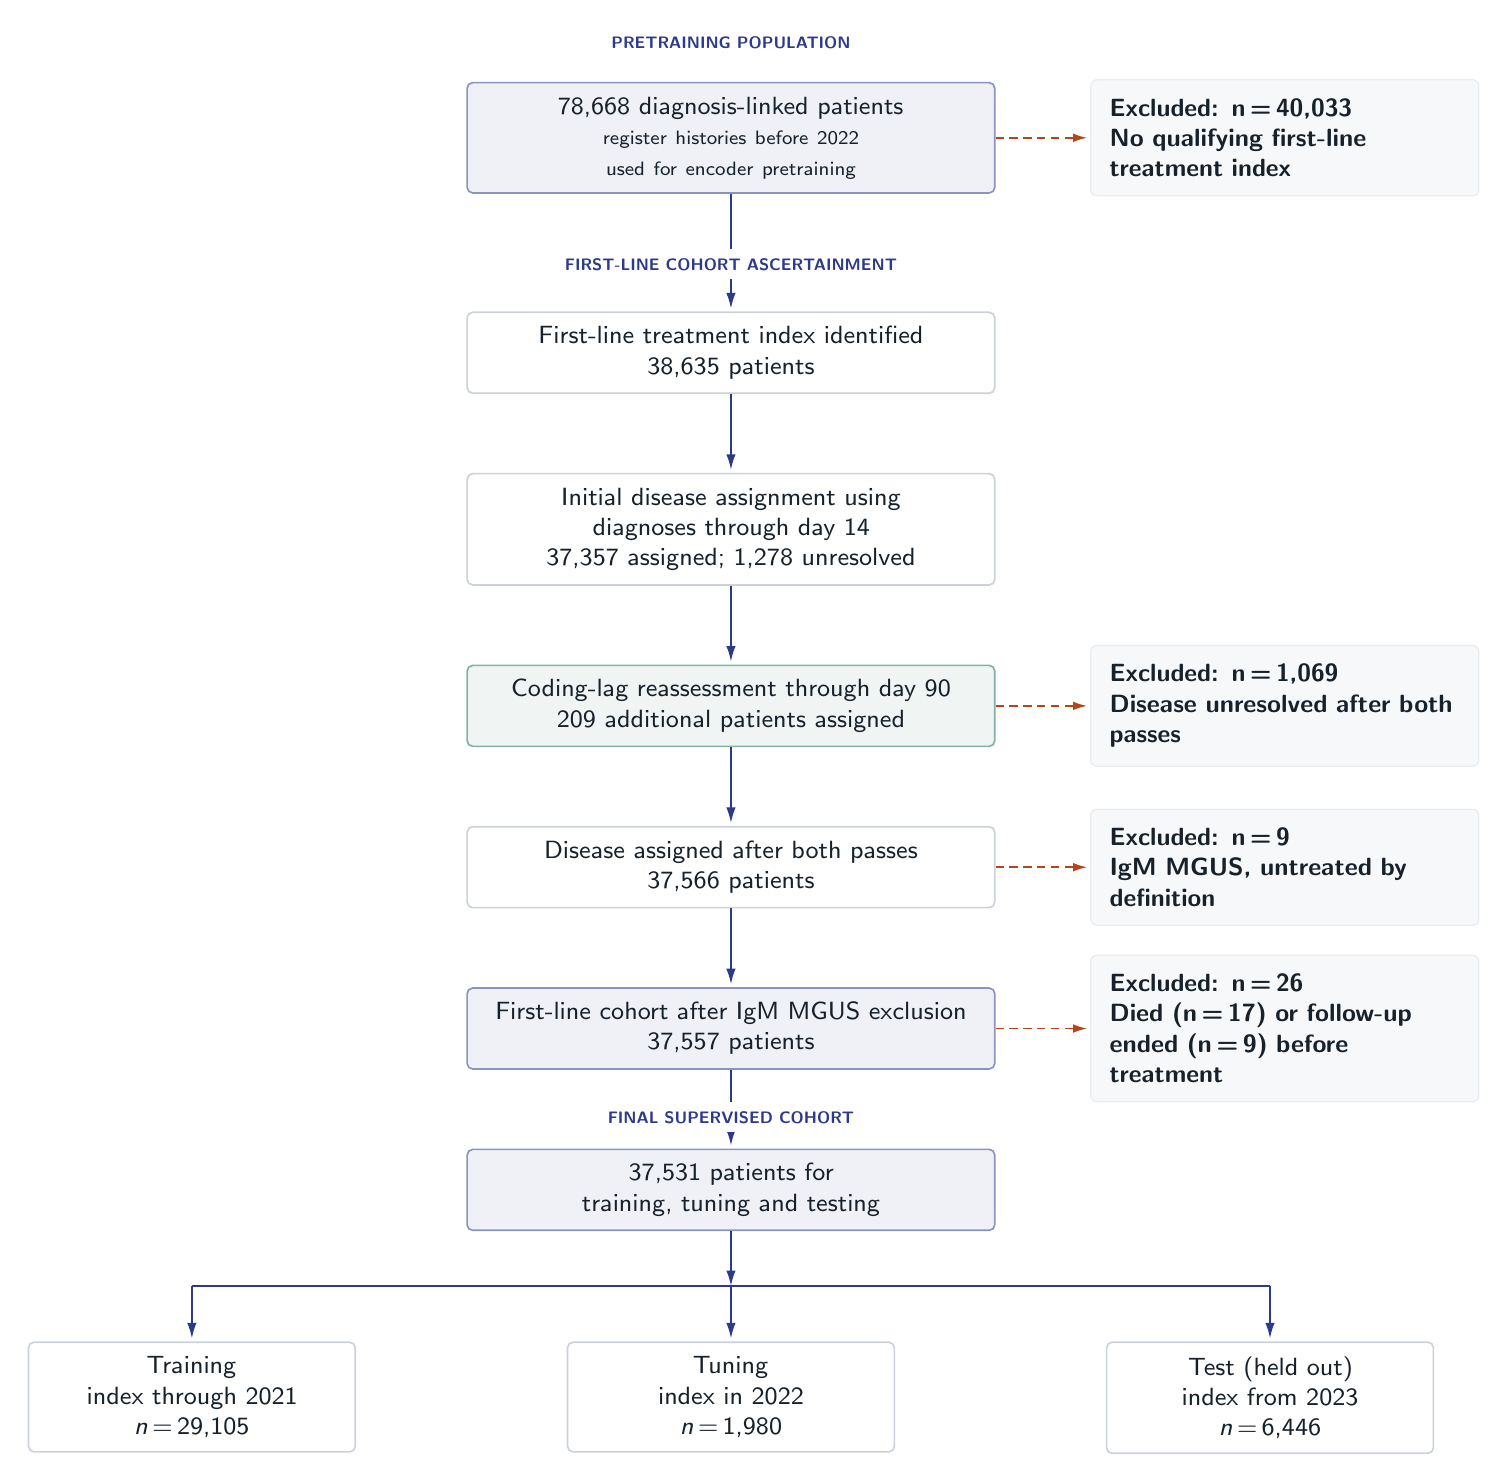
\begin{tikzpicture}[opera,node distance=10mm and 12mm,
    every node/.append style={execute at begin node={\hyphenpenalty=10000\exhyphenpenalty=10000}}]
  \node[stageblue,text width=6.1cm] (pretrainbox)
    {78,668 diagnosis-linked patients\\{\scriptsize register histories before 2022 used for encoder pretraining}};
  \node[eyebrow,above=3mm of pretrainbox] (pretrainlabel) {PRETRAINING POPULATION};
  \node[eyebrow,below=7mm of pretrainbox] (branchlabel)
    {FIRST-LINE COHORT ASCERTAINMENT};
  \node[stage,text width=6.1cm,below=4mm of branchlabel] (index)
    {First-line treatment index identified\\38,635 patients};
  \node[stage,text width=6.1cm,below=of index] (pass1)
    {Initial disease assignment using diagnoses through day 14\\37,357 assigned; 1,278 unresolved};
  \node[stageteal,text width=6.1cm,below=of pass1] (pass2)
    {Coding-lag reassessment through day 90\\209 additional patients assigned};
  \node[stage,text width=6.1cm,below=of pass2] (classified)
    {Disease assigned after both passes\\37,566 patients};
  \node[stageblue,text width=6.1cm,below=of classified] (firstline)
    {First-line cohort after IgM MGUS exclusion\\37,557 patients};
  \node[stageblue,text width=6.1cm,below=of firstline] (supervised)
    {37,531 patients for training, tuning and testing};

  \foreach \a/\b in {index/pass1,pass1/pass2,
                       pass2/classified,classified/firstline,firstline/supervised}
    \draw[flowblue,shorten >=1pt] (\a.south) -- (\b.north);
  \draw[flowblue,shorten >=1pt] (pretrainbox.south) -- (index.north);
  \node[eyebrow,fill=white,inner xsep=2mm] at (branchlabel) {FIRST-LINE COHORT ASCERTAINMENT};
  \node[eyebrow,fill=white,inner xsep=2mm,above=2mm of supervised]
    {FINAL SUPERVISED COHORT};

  % Mutually distinct exits from the central first-line flow.
  \node[softpanel,text width=4.45cm,align=left,right=of pretrainbox] (noindex)
    {\bfseries Excluded: \textit{n}\,=\,40{,}033\\No qualifying first-line treatment index};
  \node[softpanel,text width=4.45cm,align=left,right=of pass2] (unresolved)
    {\bfseries Excluded: \textit{n}\,=\,1{,}069\\Disease unresolved after both passes};
  \node[softpanel,text width=4.45cm,align=left,right=of classified] (secondary)
    {\bfseries Excluded: \textit{n}\,=\,9\\IgM MGUS, untreated by definition};
  \node[softpanel,text width=4.45cm,align=left,right=of firstline] (nosurvival)
    {\bfseries Excluded: \textit{n}\,=\,26\\Died (\textit{n}\,=\,17) or follow-up ended (\textit{n}\,=\,9) before treatment};
  \draw[relation,draw=OperaSienna,shorten >=1pt] (pretrainbox.east) -- (noindex.west);
  \draw[relation,draw=OperaSienna,shorten >=1pt] (pass2.east) -- (unresolved.west);
  \draw[relation,draw=OperaSienna,shorten >=1pt] (classified.east) -- (secondary.west);
  \draw[relation,draw=OperaSienna,shorten >=1pt] (firstline.east) -- (nosurvival.west);

  \node[stage,text width=3.55cm,below left=14mm and 14mm of supervised] (train)
    {Training\\index through 2021\\\textit{n}\,=\,29{,}105};
  \node[stage,text width=3.55cm,below=14mm of supervised] (tune)
    {Tuning\\index in 2022\\\textit{n}\,=\,1{,}980};
  \node[stage,text width=3.55cm,below right=14mm and 14mm of supervised] (held)
    {Test (held out)\\index from 2023\\\textit{n}\,=\,6{,}446};
  \coordinate (split) at ($(supervised.south)+(0,-7mm)$);
  \draw[flowblue] (supervised.south) -- (split);
  \draw[draw=OperaIndigo,line width=0.75pt]
    (train.north |- split) -- (held.north |- split);
  \foreach \dest in {train,tune,held}
    \draw[flowblue,shorten >=1pt] (\dest.north |- split) -- (\dest.north);

\end{tikzpicture}
}
\caption{\textbf{CONSORT diagram.} From all diagnosis-linked DALY-CARE patients to
the first-line cohort and its temporal split. Not every patient contributes to
every endpoint: outcome-specific eligibility, competing events and follow-up are
applied within each split.}
\label{fig:consort}
\end{figure}
\end{document}
